\documentclass[11pt]{article}
\usepackage{ucs}
\usepackage[utf8x]{inputenc}
\usepackage{geometry}
\usepackage[greek,english]{babel}
\newcommand{\en}{\selectlanguage{english}}
\newcommand{\gr}{\selectlanguage{greek}}
\usepackage{amsmath}
\usepackage{amssymb}
\usepackage{mathtools}
\usepackage{float}
\usepackage{graphicx}
\usepackage{a4wide}


\usepackage{tikz}
\usepackage{titlesec}
\usepackage{caption}
\setcounter{secnumdepth}{4}
\usepackage[bottom]{footmisc}

\usepackage{xcolor} % colors
\usepackage[toc,page]{appendix} % for appendices
\usepackage{csquotes} % for quotes
\usepackage{cancel} % for canceling values to zero

\allowdisplaybreaks % allows split between pages

\DeclarePairedDelimiter{\ceil}{\lceil}{\rceil}
\DeclarePairedDelimiter\floor{\lfloor}{\rfloor}
\usepackage{wrapfig} % wrap text to figure


%\usepackage{fancyhdr} % for header
%\pagestyle{fancy}
%\fancyhf{}
%\fancyfoot[C]{\thepage} % centere number of page
%%\fancyhead[R]{\rightmark}
\usepackage{bm} % BOLD

\usepackage{listings}

\usepackage{caption}
\usepackage{subcaption}
%\usepackage{algorithmic} % for algorithms
\usepackage[ruled,vlined]{algorithm2e}

\newcommand{\approxtext}[1]{\ensuremath{\stackrel{\text{#1}}{\approx}}}
%\renewcommand{\footrulewidth}{0.4pt}% default is 0pt

\usepackage[framed]{matlab-prettifier}
\newcommand\numberthis{\addtocounter{equation}{1}\tag{\theequation}}
\renewcommand{\lstlistingname}{Code}


\usepackage{optidef}
\usepackage{hyperref}
\usepackage{enumitem}

\hypersetup{
	colorlinks   = true, %Colours links instead of ugly boxes
	urlcolor     = blue, %Colour for external hyperlinks
	linkcolor    = blue, %Colour of internal links
	citecolor   = red %Colour of citations
}

\setlength{\parskip}{1em}
\DeclareMathOperator*{\argmax}{argmax} % FOR ARGMAX
\DeclareMathOperator*{\argmin}{argmin} % FOR ARGMIN
\DeclareMathOperator{\tr}{tr}
\DeclareMathOperator{\mean}{E}
\DeclareMathOperator{\rank}{rank}
\DeclareMathOperator{\diag}{diag}
\DeclareMathOperator{\sgn}{sgn}

\begin{document}
	\begin{titlepage}
		\title{\hrulefill\\
			\vspace{5mm}
			{\Huge \textbf{First iteration of K-Means clustering algorithm using MapReduce}} \\ \hrulefill\\
			\vspace{10mm}
			{\Large {{Assignment 2}
		}}}
		\author{Panourgia Evangelia (t8190130)\\
			Papadatos Ioannis (t8190314)\\
			Professor: Chatziantoniou Damianos}
		\date{Latest Update: \today}
		\maketitle
		
		\thispagestyle{empty}
		\begin{center}
			
\includegraphics[width=0.3\textwidth]{./aueblogo.jpg}\\
			\vspace{10mm}
			School of Management Science and Technology,\\ Athens University of Economics and Business
		\end{center}
	\end{titlepage}
	\noindent
	
	\tableofcontents	
	
	\newpage
	\section{Hadoop Installation}
	As far as the installation of Hadoop, we decided to use Hadoop through a Virtual Machine. We chose to download Bitnami's Virtual Machine image for Hadoop [1], because it is lightweight and easy to use. Then, we launched a Virtual Machine by importing the downloaded image to the Oracle VirtualBox [2] virualization application. Once the startup process was completed, we logged in using the login prompt shown in the image below in order to access the console. Afterwards, we installed git (command: sudo apt install git) at the Virtual Machine through the console, in order to clone our Github repository containing the code. Finally, we also installed pip3 (command: sudo apt install python3-pip) in order to install the dependencies used in our code which are listed in the requirements.txt file (command: pip3 install -r requirements.txt).
	 
	 
	\begin{figure}[H]
		\makebox[\textwidth][c]{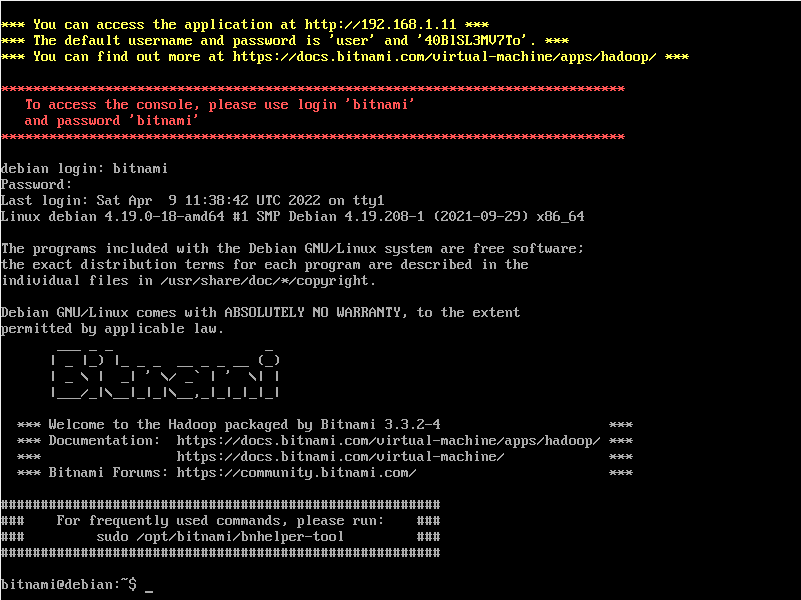
\includegraphics[width=.7\textwidth]{figs/img/install_bitnami.png}}
		\caption{Install Bitnami}
	\end{figure}

	
	\newpage
	\section{Dataset Creation}
	The script generate\_data.py was written for generating data-points in the form (x, y). Specifically, it reads centroids in the form (x, y) from a csv file (-i) and generates the specified amount of data-points around each centroid (-n), which is then written to the specified file (-o). The argument -d is optional, but if provided it generates the graphical representation of the points in an image (points.png).
	
	\begin{figure}[H]
		\makebox[\textwidth][c]{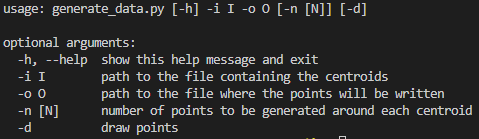
\includegraphics[width=.7\textwidth]{figs/img/cmd3.png}}
		\caption{Script arguments.}
	\end{figure}	

	For our assignment needs, the script described above was used with the command shown below to read three centroids from the centroids.csv file and generate 600.000 data-points around each one of them, that was then written to the points.csv file. Also the points.png image was produced since the argument -d was provided.    
	
	\begin{figure}[H]
		\makebox[\textwidth][c]{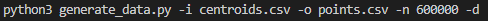
\includegraphics[width=.7\textwidth]{figs/img/cmd5.png}}
		\caption{Dataset generation command.}
	\end{figure}        
	
	\begin{figure}[H]
		\makebox[\textwidth][c]{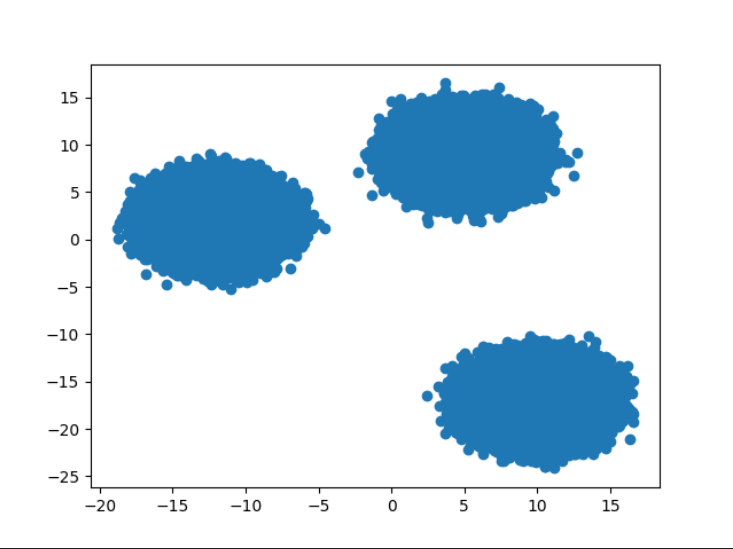
\includegraphics[width=.7\textwidth]{figs/img/plot.png}}
		\caption{Dataset graphical representation.}
	\end{figure} 
	 
	
	\begin{figure}[H]
		\makebox[\textwidth][c]{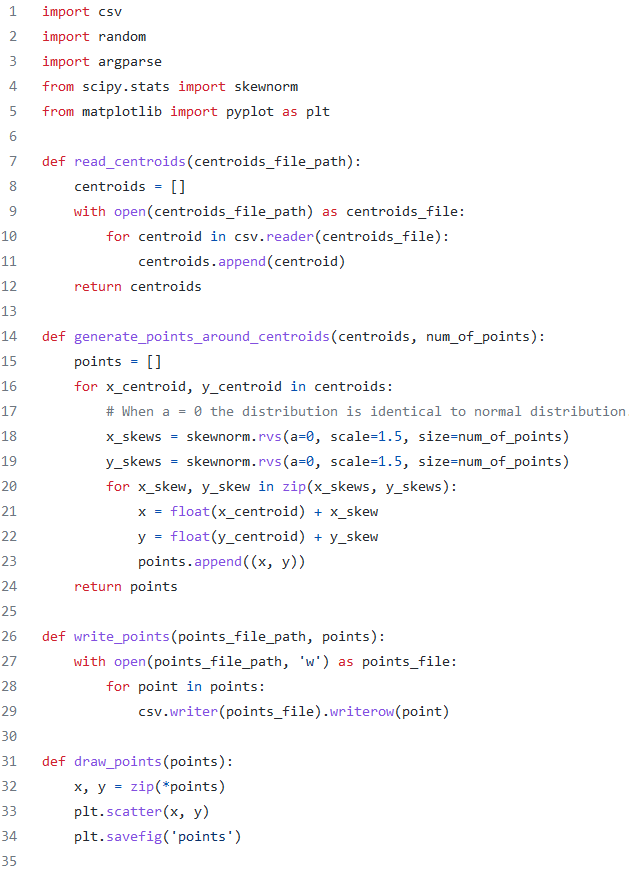
\includegraphics[width=.7\textwidth]{figs/img/datagen_1.png}}
		\caption{generate\_data.py source code.}
	\end{figure}
	
\begin{figure}[H]
		\makebox[\textwidth][c]{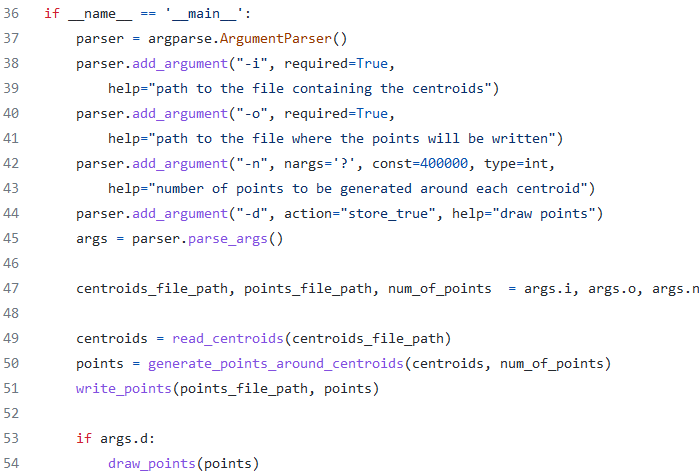
\includegraphics[width=.7\textwidth]{figs/img/datagen_2.png}}
		\caption{generate\_data.py source code.}
	\end{figure}

	\newpage
	\section{K-Means Clustering Algorithm}
	
The script kmeans.py was written to implement the first iteration of the K-Means clustering algorithm [6] using MapReduce. To write the MapReduce job we used the Python library mrjob [3].

The configure\_args method is used to add a file argument that allows the user to specify the path to the file containing the initial centroids:

\begin{figure}[H]
		\makebox[\textwidth][c]{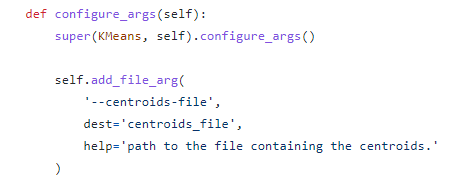
\includegraphics[width=.7\textwidth]{figs/img/configureArgs.png}}
		\caption{configure\_args method}
	\end{figure}

	The load\_centroids method is used to broadcast the initial centroids to the mappers:
	
	\begin{figure}[H]
		\makebox[\textwidth][c]{\includegraphics[width=.7\textwidth]{figs/img/load\_centroids.png}}
		\caption{load\_centroids method}
	\end{figure}

\newpage
The mapper method is used to map each point to its closest centroid based on euclidean distance:
\begin{figure}[H]
		\makebox[\textwidth][c]{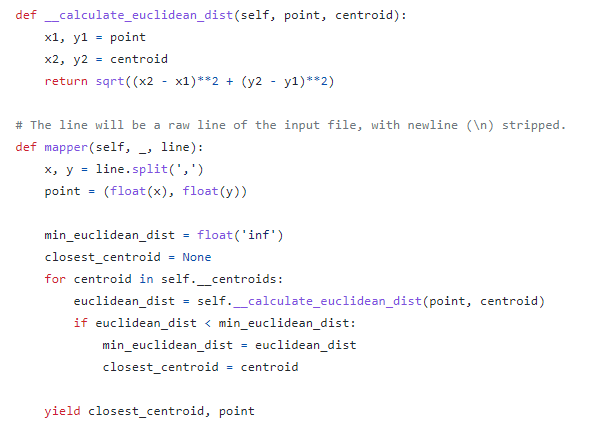
\includegraphics[width=.7\textwidth]{figs/img/mapper.png}}
		\caption{mapper method}
	\end{figure}
	The reducer method is used to compute the new centroids based on the data points that were mapped to each centroid:
	\begin{figure}[H]
		\makebox[\textwidth][c]{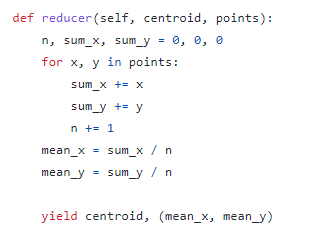
\includegraphics[width=.7\textwidth]{figs/img/reducer.png}}
		\caption{reducer method}
	\end{figure}
	
	\begin{figure}[H]
		\makebox[\textwidth][c]{
\includegraphics[width=.7\textwidth]{figs/img/cmd4.png}}
		\caption{MapReduce job execution command}
	\end{figure}
	
	

	
	
\begin{figure}[H]
		\makebox[\textwidth][c]{\includegraphics[width=.7\textwidth]{figs/img/new\_centroids.png}}
		\caption{MapReduce job results}
	\end{figure}
	
	We observe that the deviation between the initial and the new centroids is small, which is normal since the data points were generated around the initial centroids using normal distribution.
	
	\begin{figure}[H]
		\makebox[\textwidth][c]{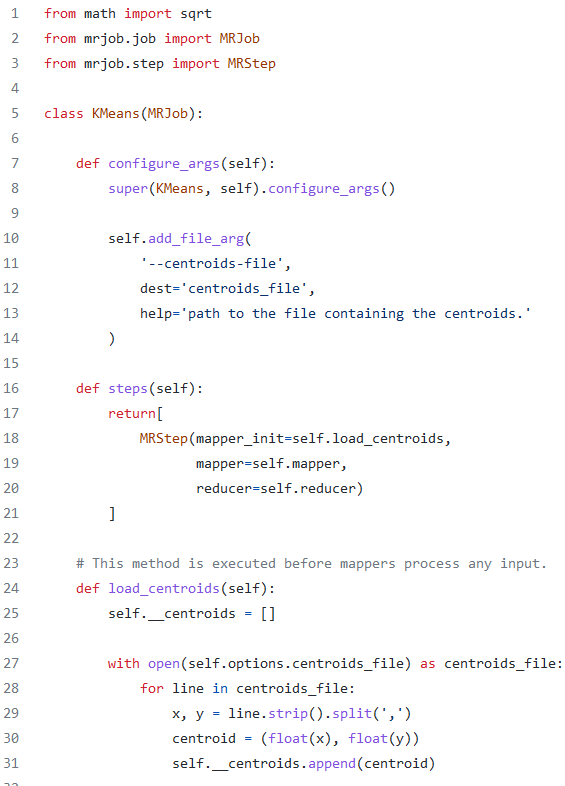
\includegraphics[width=.7\textwidth]{figs/img/kmeans_1.png}}
		\caption{kmeans.py source code.}
	\end{figure}
	
	\begin{figure}[H]
		\makebox[\textwidth][c]{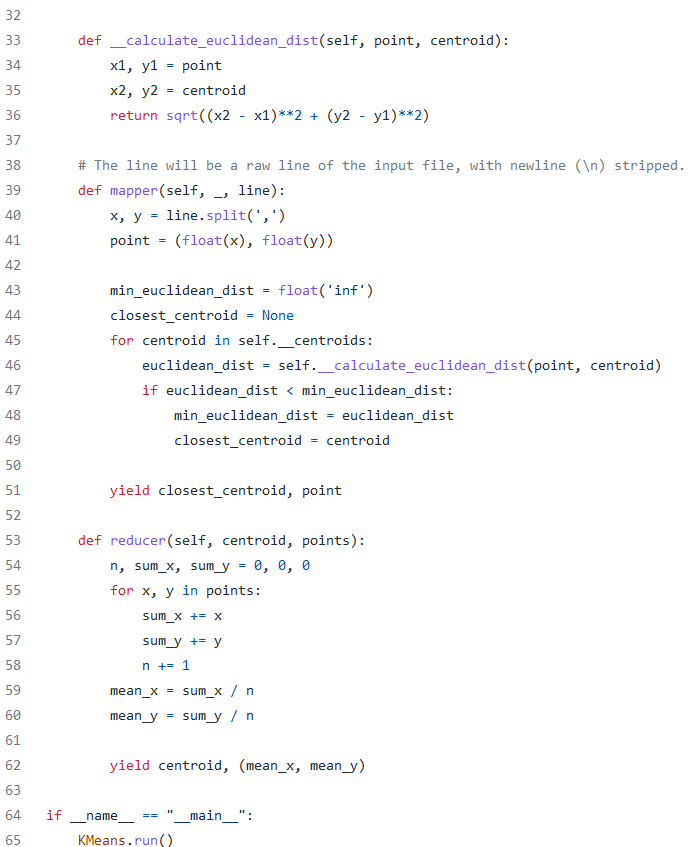
\includegraphics[width=.7\textwidth]{figs/img/kmeans_2.png}}
		\caption{kmeans.py source code.}
	\end{figure}
	
	\newpage
	\begin{thebibliography}{1}
		\bibitem{beck}
		Hadoop packaged by Bitnami, \textit{\textbf{https://bitnami.com/stack/hadoop/virtual-machine}}
	
	
		\bibitem{beck}
		Oracle VirtualBox, \textit{\textbf{https://www.virtualbox.org/}}

		
		\bibitem{beck}
		mrjob, \textit{\textbf{https://pypi.org/project/mrjob/}}
		
		\bibitem{beck}
		skewnorm, \textit{\textbf{https://docs.scipy.org/doc/scipy/reference/generated/scipy.stats.skewnorm.html}}
		
		\bibitem{beck}
		matplotlib, \textit{\textbf{https://matplotlib.org/}}
		
		\bibitem{beck}{MapReduce Algorithms for k-means Clustering ,
  		title = {MapReduce Algorithms for k-means Clustering},
  		author = {Max Bodoia},
  		note  =  {\url{https://stanford.edu/~rezab/classes/cme323/S16/projects_reports/bodoia.pdf}},
  		note = {Accessed: 10-4-2022},
}
		
		
	\end{thebibliography}
	
	
\end{document}